\documentclass[tikz,border=10pt]{standalone}
\usepackage{circuitikz}
\usepackage{xcolor}
\usepackage{amsmath}
\usetikzlibrary{arrows}

\begin{document}
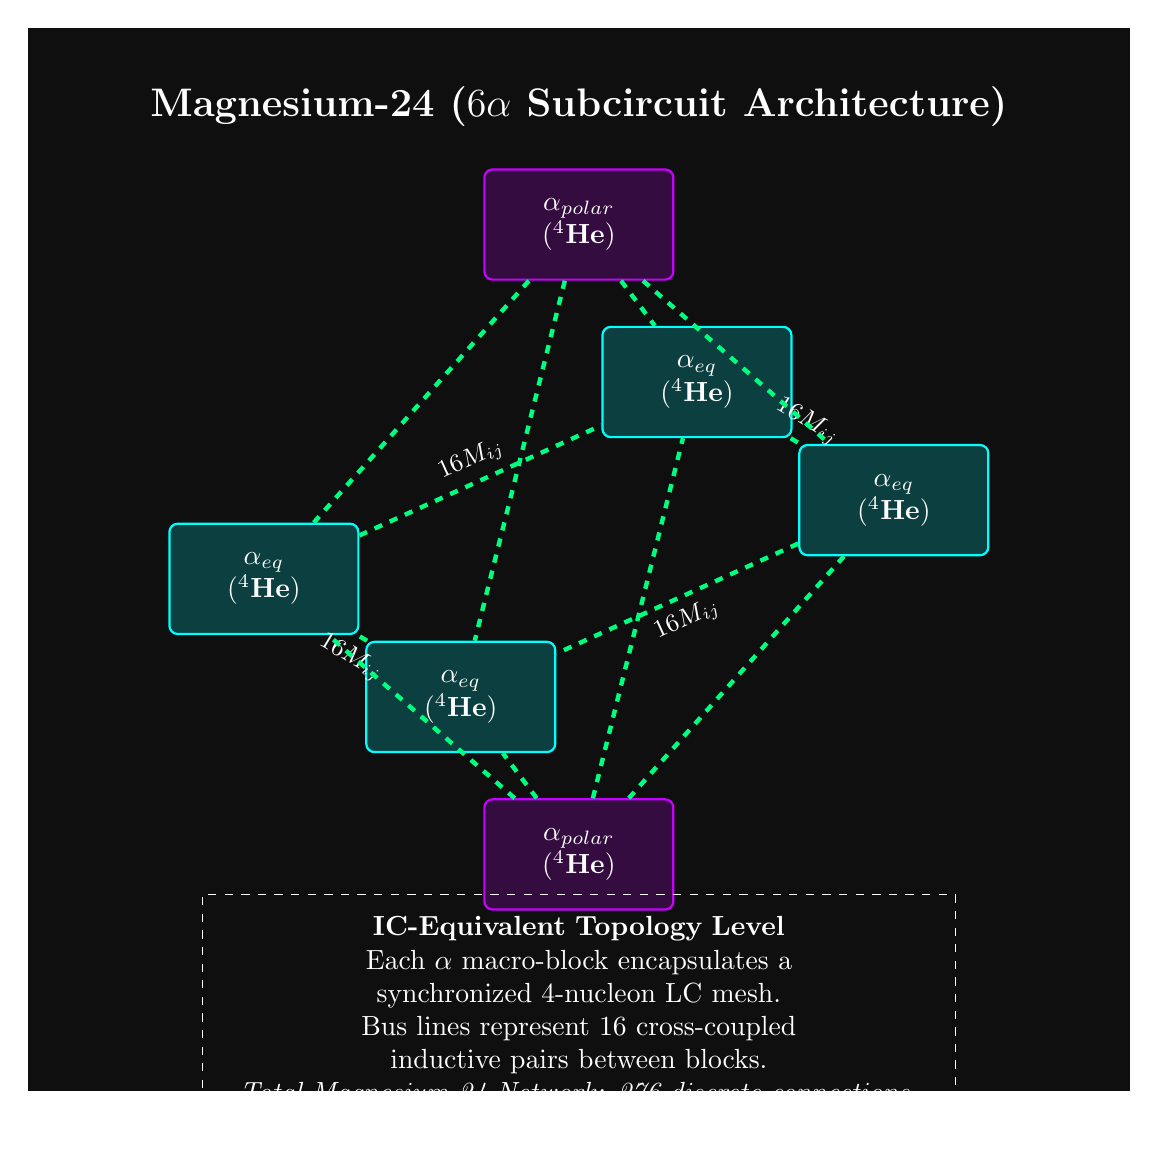
\begin{tikzpicture}[>=latex']

\definecolor{neonblue}{RGB}{0, 255, 255}
\definecolor{neongreen}{RGB}{0, 255, 128}
\definecolor{darkbg}{RGB}{15, 15, 15}
\definecolor{neonpurple}{RGB}{200, 0, 255}

% Fill background
\fill[darkbg] (-7,-7) rectangle (7,6.5);

% Title
\node[text=white, font=\bfseries\Large] at (0, 5.5) {Magnesium-24 ($6\alpha$ Subcircuit Architecture)};

\tikzset{
    alpha block/.style={
        draw=#1, thick, fill=darkbg!80!#1,
        rectangle, rounded corners=3pt,
        minimum width=2.4cm, minimum height=1.4cm,
        text=white, font=\bfseries, align=center
    },
    bus/.style={
        draw=neongreen, ultra thick, dashed
    }
}

% ISOMETRIC EQUATORIAL PLANE (4 Alphas)
\node[alpha block=neonblue] (EW) at (-4, -0.5) {$\alpha_{eq}$\\$(^4\text{He})$};
\node[alpha block=neonblue] (EE) at (4, 0.5) {$\alpha_{eq}$\\$(^4\text{He})$};
\node[alpha block=neonblue] (EN) at (1.5, 2.0) {$\alpha_{eq}$\\$(^4\text{He})$};
\node[alpha block=neonblue] (ES) at (-1.5, -2.0) {$\alpha_{eq}$\\$(^4\text{He})$};

% POLAR AXIS (2 Alphas)
\node[alpha block=neonpurple] (P1) at (0, 4.0) {$\alpha_{polar}$\\$(^4\text{He})$};
\node[alpha block=neonpurple] (P2) at (0, -4.0) {$\alpha_{polar}$\\$(^4\text{He})$};

% --- MACRO-COUPLINGS (BUS LINES) ---

% Equatorial Ring
\draw[bus] (EW) -- (EN) node[midway, sloped, above, text=white, font=\small] {$16 M_{ij}$};
\draw[bus] (EN) -- (EE) node[midway, sloped, above, text=white, font=\small] {$16 M_{ij}$};
\draw[bus] (EE) -- (ES) node[midway, sloped, below, text=white, font=\small] {$16 M_{ij}$};
\draw[bus] (ES) -- (EW) node[midway, sloped, below, text=white, font=\small] {$16 M_{ij}$};

% Polar North to Equator
\draw[bus] (P1) -- (EW);
\draw[bus] (P1) -- (EE);
\draw[bus] (P1) -- (EN);
\draw[bus] (P1) -- (ES);

% Polar South to Equator
\draw[bus] (P2) -- (EW);
\draw[bus] (P2) -- (EE);
\draw[bus] (P2) -- (EN);
\draw[bus] (P2) -- (ES);

% Legend
\node[text=white, text width=9cm, align=center, draw=white, dashed, inner sep=8pt] at (0, -6) {
    \textbf{IC-Equivalent Topology Level}\\
    Each $\alpha$ macro-block encapsulates a synchronized 4-nucleon LC mesh.\\
    Bus lines represent 16 cross-coupled inductive pairs between blocks.\\
    \textit{Total Magnesium-24 Network: 276 discrete connections.}
};

\end{tikzpicture}
\end{document}
